\chapter{Essay: How a Pilot Uses Vectors}

% CHILD SECTION END 



% CHILD SECTION START 

How an air traffic controller uses radar

% CHILD SECTION END 



% CHILD SECTION START 

How sonar is used for fishing

% CHILD SECTION END 



% CHILD SECTION START 

\essayauthorblurb[Asogan Moodaly received his Bachelor of Science
degree (with honours) in Mechanical Engineering from the University
of Natal, Durban in South Africa. For his final year design project
he worked on a 3-axis filament winding machine for composite (Glass
re-enforced plastic in this case) piping. He worked in Vereeniging,
Gauteng at Mine Support Products (a subsidiary of Dorbyl Heavy
Engineering) as the design engineer once he graduated. He currently
lives in the Vaal Triangle area and is working for Sasol Technology
Engineering as a mechanical engineer, ensuring the safety and
integrity of equipment installed during projects.]

\essaytitle[Pressure and Forces]

In the mining industry, the roof (hangingwall) tends to drop as the
face of the tunnel (stope) is excavated for rock containing gold.

As one can imagine, a roof falling on one's head is not a nice
prospect! Therefore the roof needs to be supported.
\begin{figure}[H]
\centering
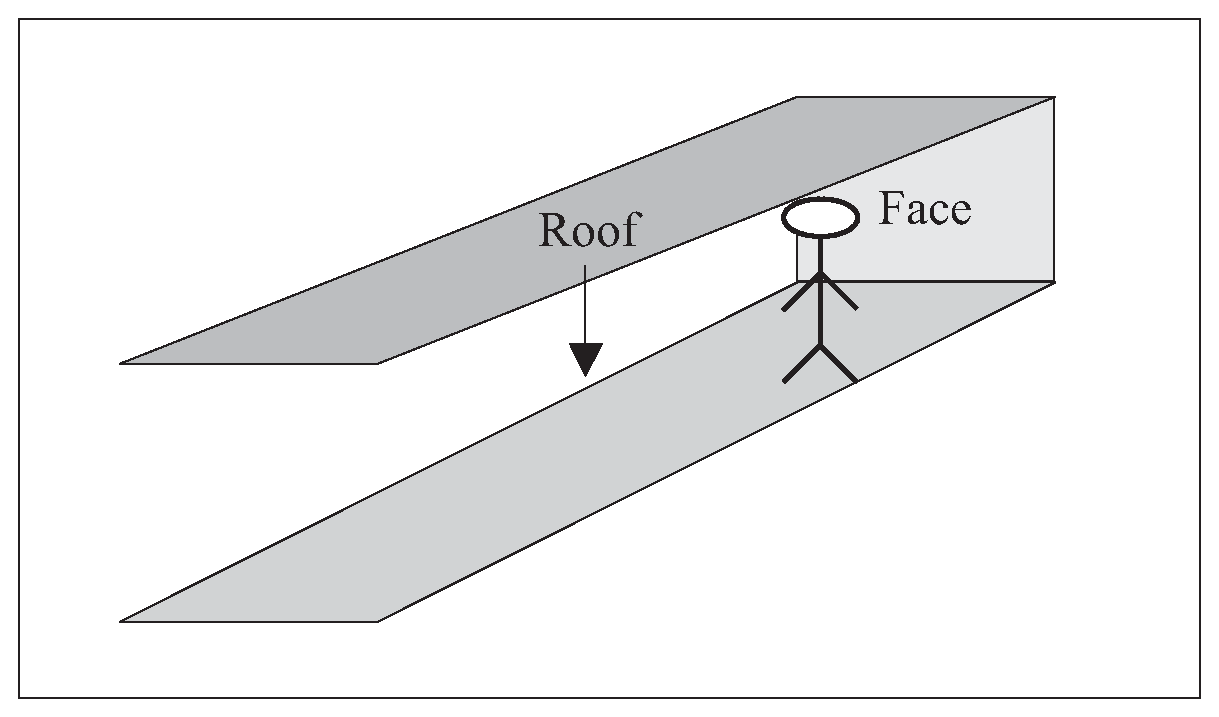
\includegraphics[scale=0.4]{../../epsimages/EssayPressure1.eps}
\end{figure}

The roof is not one big uniform chunk of rock. Rather it is broken
up into smaller chunks. It is assumed that the biggest chunk of rock
in the roof has a mass of less than 20 000 kgs therefore each
support has to be designed to resist a force related to that mass.
The strength of the material (either wood or steel) making up the
support is taken into account when working out the minimum required
size and thickness of the parts to withstand the force of the roof.

\begin{figure}[H]
\centering
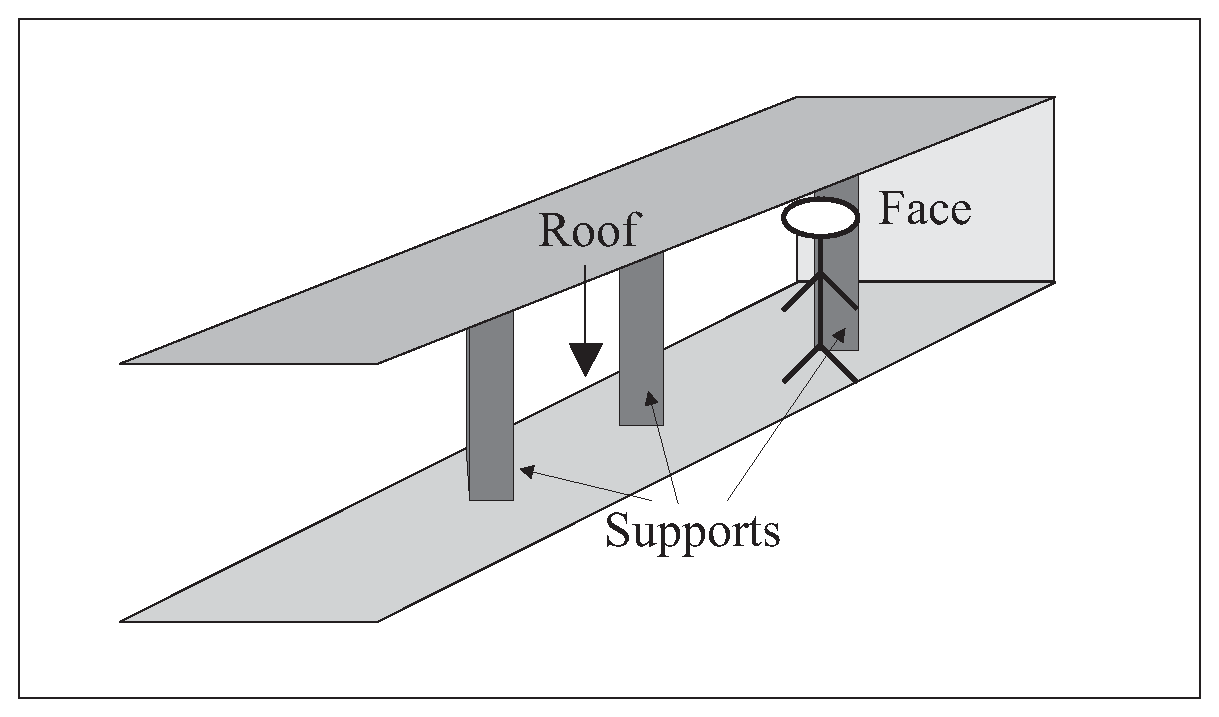
\includegraphics[scale=0.4]{../../epsimages/EssayPressure2.eps}
\end{figure}


Sometimes the design of the support is such that the support needs
to withstand the rock mass without the force breaking the roof..

Therefore hydraulic supports (hydro = water) use the principles of
force and pressure such that as a force is exerted on the support,
the water pressure increases. A pressure relief valve then squirts
out water when the pressure (and thus the force) gets too large.
Imagine a very large, modified doctor's syringe.
\begin{figure}[H]
\centering
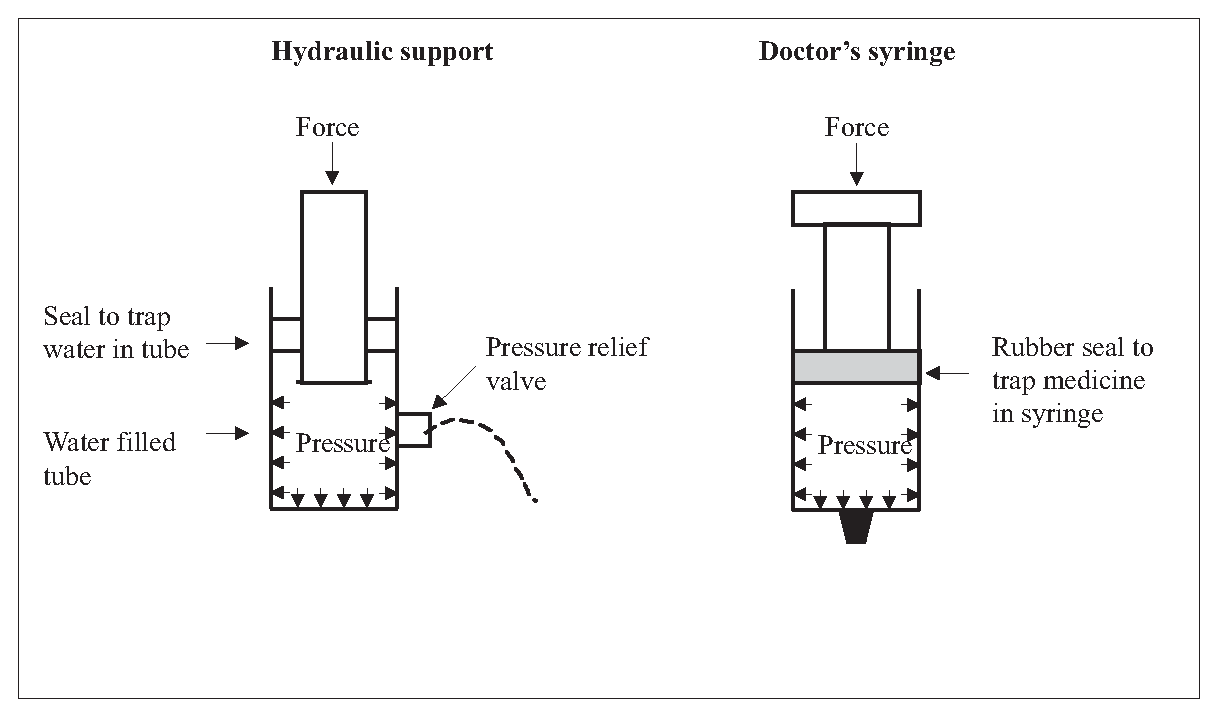
\includegraphics[scale=0.4]{../../epsimages/EssayPressure3.eps}
\end{figure}

In the petrochemical industry, there are many vessels and pipes that
are under high pressures. A vessel is a containment unit (Imagine a
pot without handles, that has the lid welded to the pot  that would
be a small vessel) where chemicals mix and react to form other
chemicals, amongst other uses.
\begin{figure}[H]
\centering
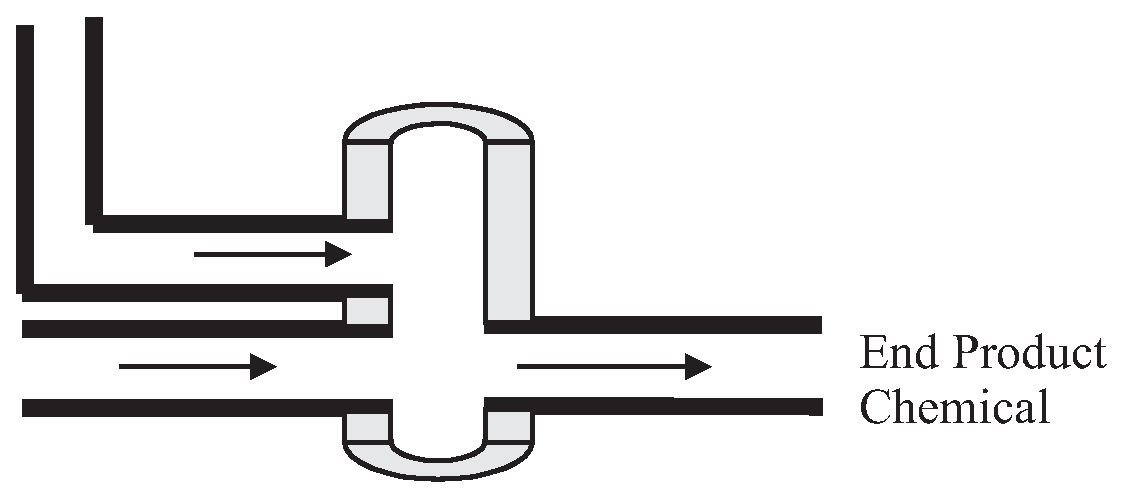
\includegraphics[scale=0.4]{../../epsimages/EssayPressure4.eps}
\end{figure}

The end product chemicals are sold to companies that use these
chemicals to make shampoo, dishwashing liquid, plastic containers,
fertilizer, etc. Anyway, some of these chemical reactions require
high temperatures and pressures in order to work. These pressures
result in forces being applied to the insides of the vessels and
pipes. Therefore the minimum thickness of the pipe and vessels walls
must be determined using calculations, to withstand these forces.
These calculations take into account the strength of the material
(typically steel, plastic or composite), the diameter and of course
the pressure inside the equipment. Let examine the concepts of
force and pressure in further detail.

